\documentclass{article}

\usepackage{amsthm}
\usepackage{amsfonts}
\usepackage{amsmath}
\usepackage{amssymb}
\usepackage{fullpage}
\usepackage{graphicx}
\usepackage[usenames]{color}
\usepackage{hyperref}
  \hypersetup{
    colorlinks = true,
    urlcolor = blue,       % color of external links using \href
    linkcolor= blue,       % color of internal links 
    citecolor= blue,       % color of links to bibliography
    filecolor= blue,        % color of file links
    }
    
\usepackage{listings}

\definecolor{dkgreen}{rgb}{0,0.6,0}
\definecolor{gray}{rgb}{0.5,0.5,0.5}
\definecolor{mauve}{rgb}{0.58,0,0.82}

\lstset{frame=tb,
  language=haskell,
  aboveskip=3mm,
  belowskip=3mm,
  showstringspaces=false,
  columns=flexible,
  basicstyle={\small\ttfamily},
  numbers=none,
  numberstyle=\tiny\color{gray},
  keywordstyle=\color{blue},
  commentstyle=\color{dkgreen},
  stringstyle=\color{mauve},
  breaklines=true,
  breakatwhitespace=true,
  tabsize=3
}

\theoremstyle{theorem} 
   \newtheorem{theorem}{Theorem}[section]
   \newtheorem{corollary}[theorem]{Corollary}
   \newtheorem{lemma}[theorem]{Lemma}
   \newtheorem{proposition}[theorem]{Proposition}
\theoremstyle{definition}
   \newtheorem{definition}[theorem]{Definition}
   \newtheorem{example}[theorem]{Example}
\theoremstyle{remark}    
  \newtheorem{remark}[theorem]{Remark}


\title{CPSC-402 Report\\Compiler Construction}
\author{Connor Cowher  \\ Chapman University}

\date{\today}

\begin{document}

\maketitle

\begin{abstract}
Short  summary of purpose and content.  
\end{abstract}
\clearpage

\tableofcontents
\clearpage

\section{Introduction}\label{intro}

~~~~~~Section~\ref{intro} Come back to this~~~~~~

\subsection{General Remarks}
\medskip\noindent

\begin{definition} 
This is a definition.
\end{definition}

\begin{example}
This is an example.
\end{example}

\begin{proposition}
This is a proposition.
\end{proposition}

\begin{theorem}
This is a theorem.
\end{theorem}

\noindent You can also create your own environment, eg if you want to have Question, Notation, Conjecture, etc.

\section{Homework}\label{homework}

This section contains my solutions to the homework. 

\subsection{Week 1}

\medskip\begin{center}
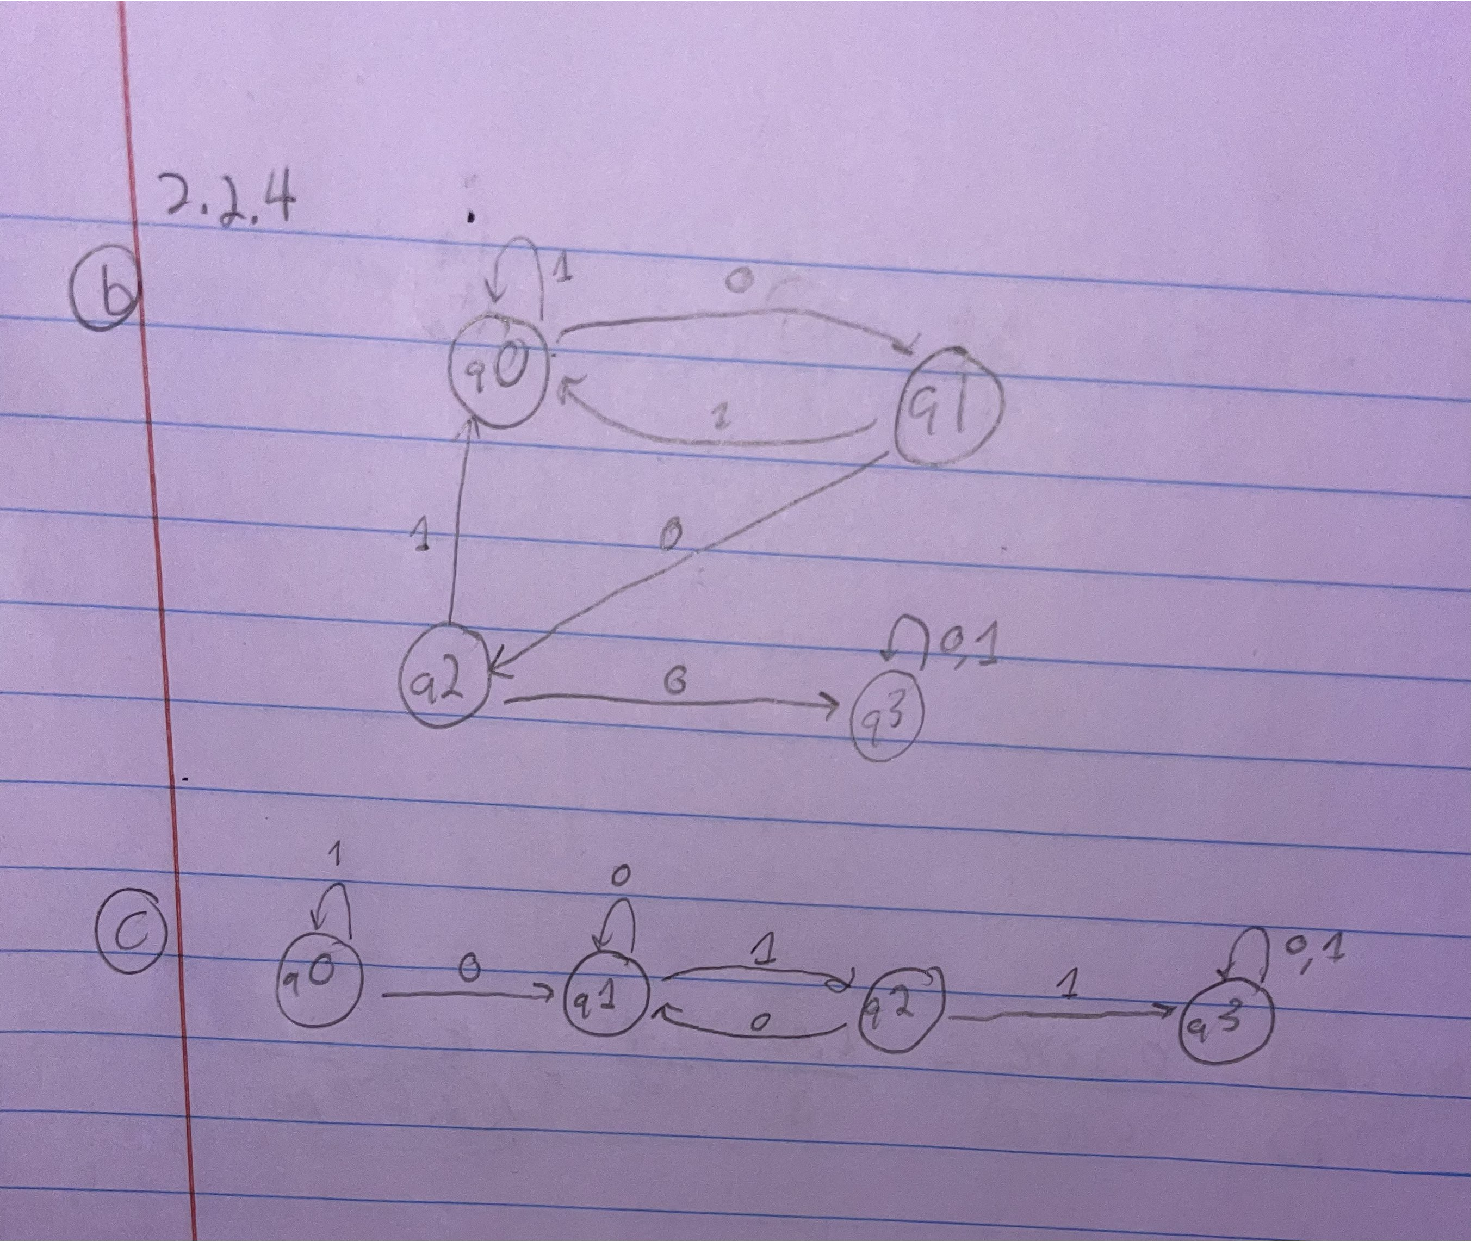
\includegraphics[width=15cm, height=17.5cm]{Week1.pdf}
\end{center}

\subsection{Week 2}

\medskip\begin{center}
\includegraphics[width=15cm, height=20cm]{Week2 (2).pdf}
\end{center}
\clearpage

\subsection{Week 3}
Converting NFAs to DFAs by Hand
\medskip\begin{center}
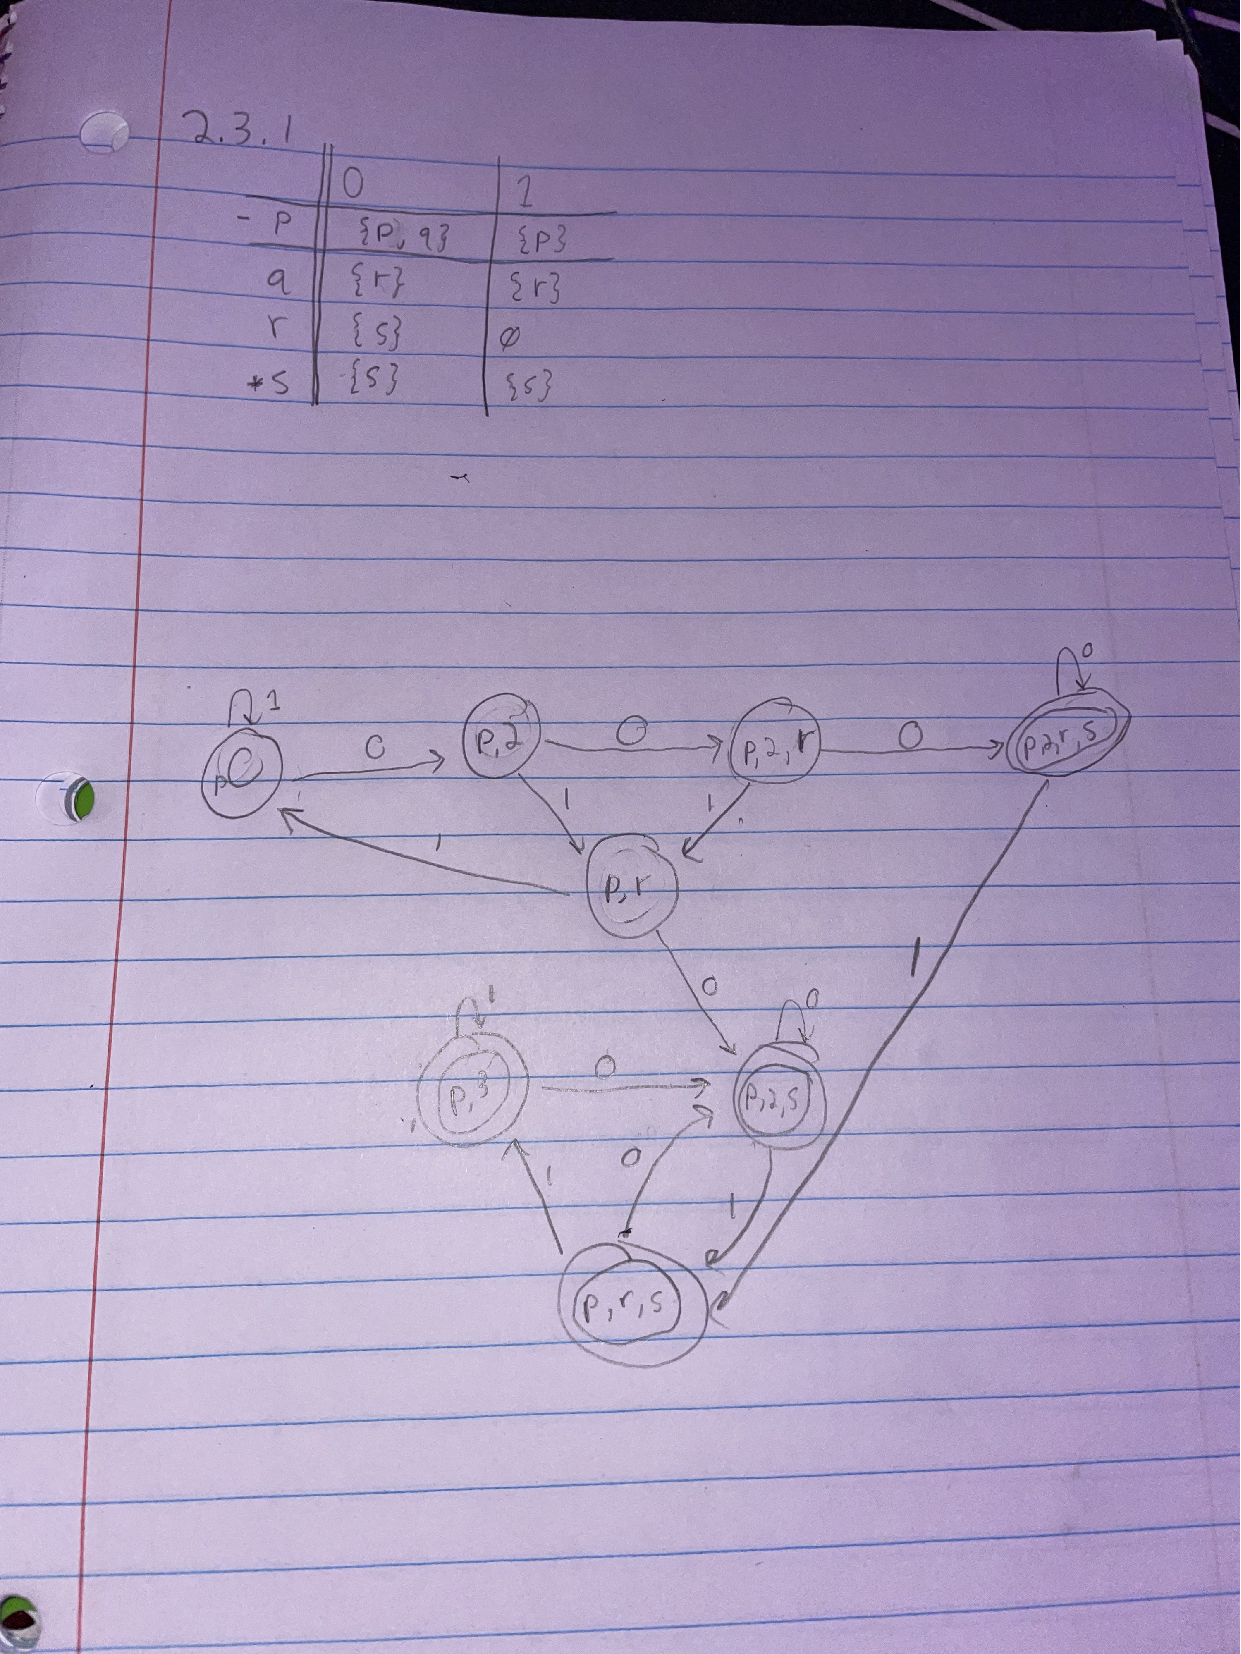
\includegraphics[width=15cm, height=20cm]{Week3.pdf}
\end{center}
\clearpage

Converting NFAs to DFAs In Haskell Using the List Monad
\medskip\begin{center}
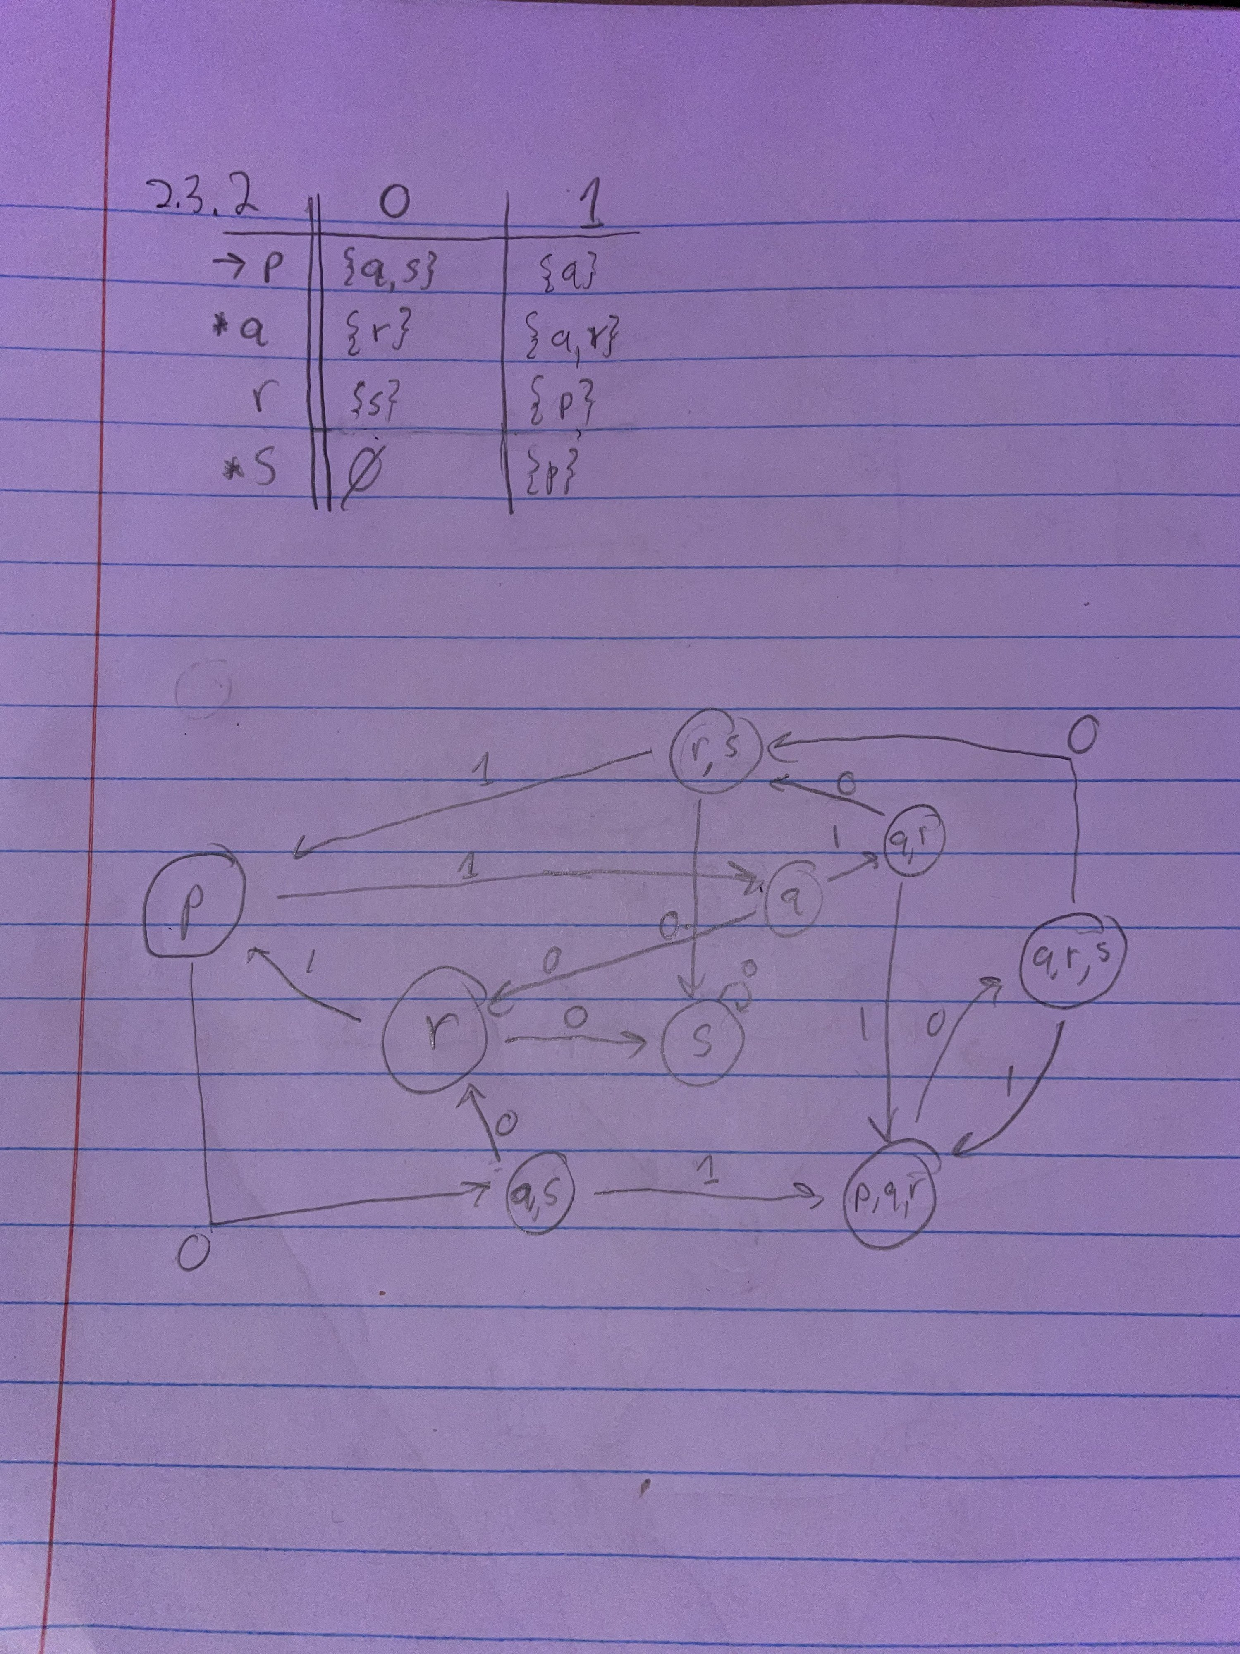
\includegraphics[width=15cm, height=20cm]{Week3P2.pdf}
\end{center}
\clearpage

\subsection{Week4}
Write out the concrete syntax tree for the complete Fibonacci program.
\medskip\begin{center}
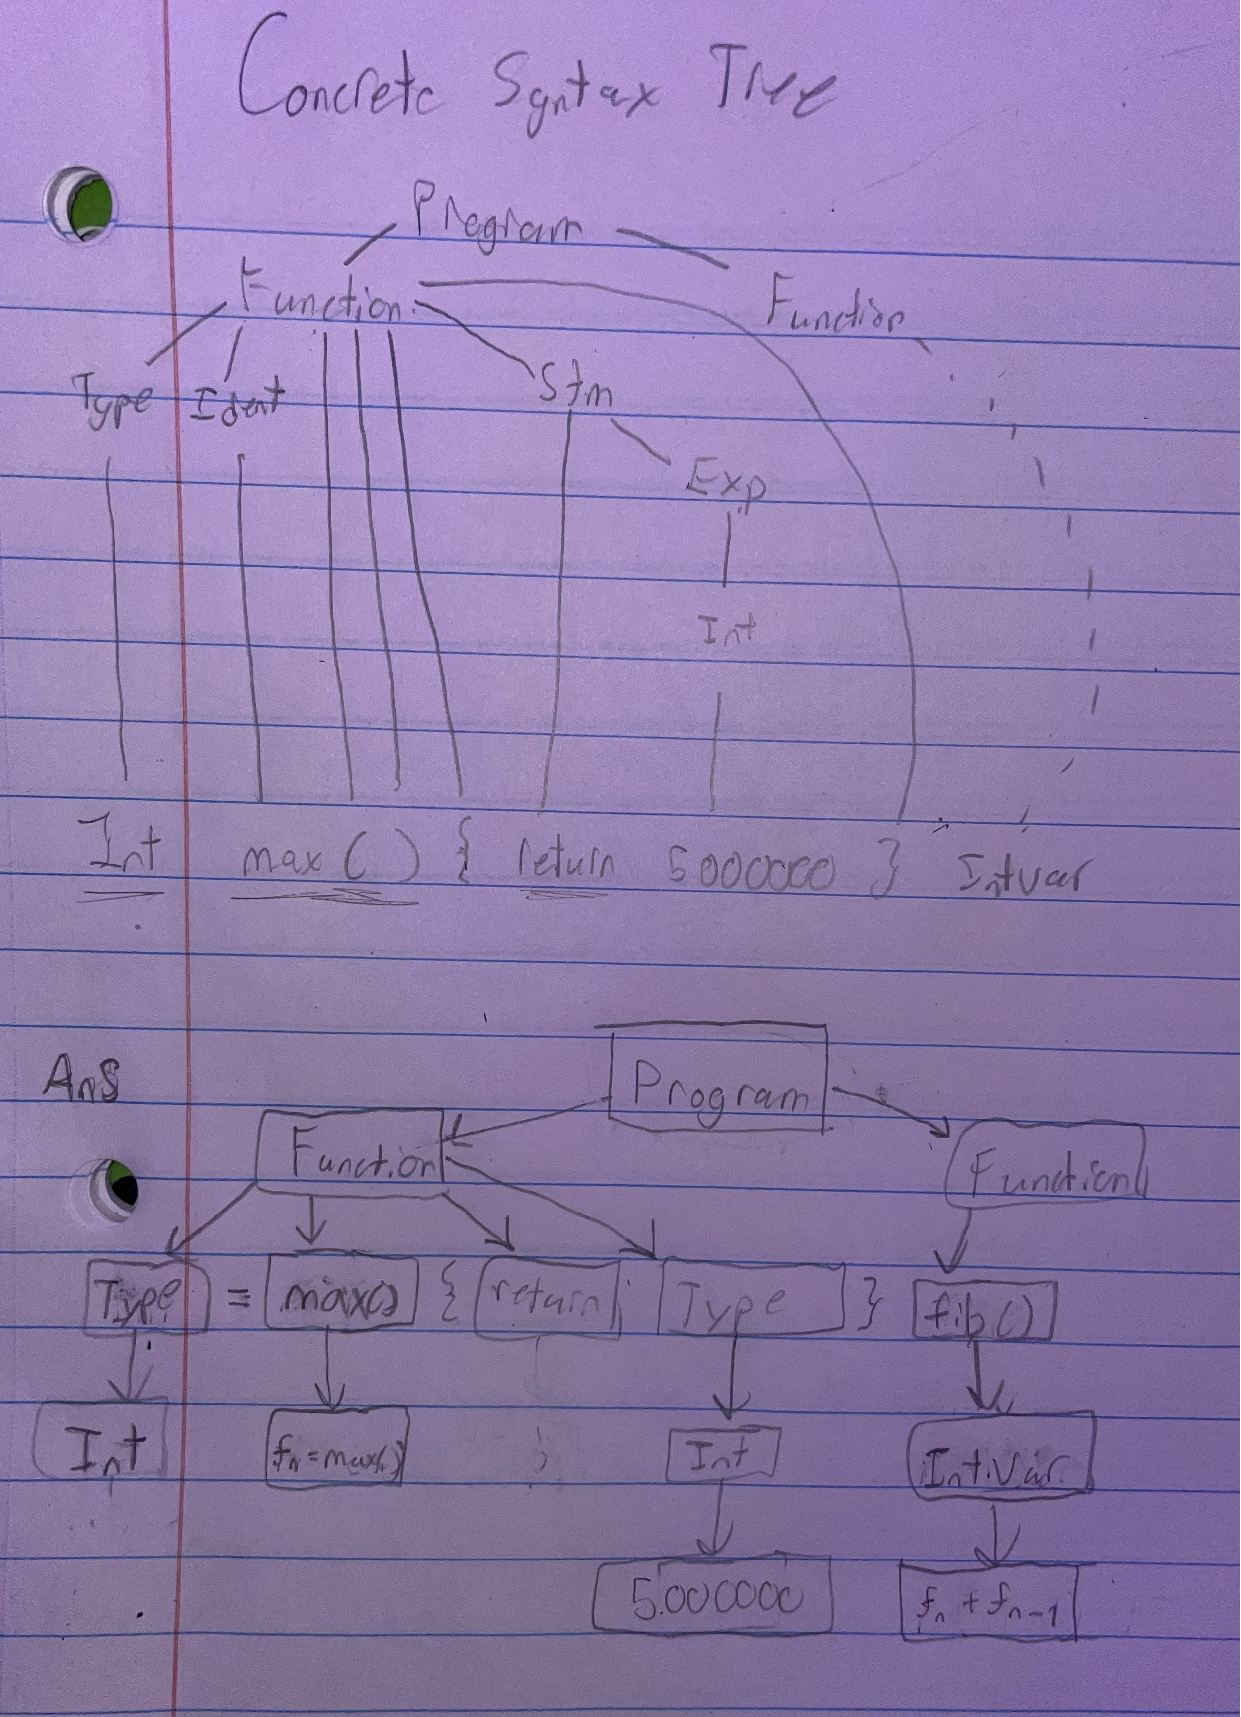
\includegraphics[width=15cm, height=20cm]{Week4P1.pdf}
\end{center}
\clearpage

Write out the abstract syntax tree for the complete Fibonacci program.
\medskip\begin{center}
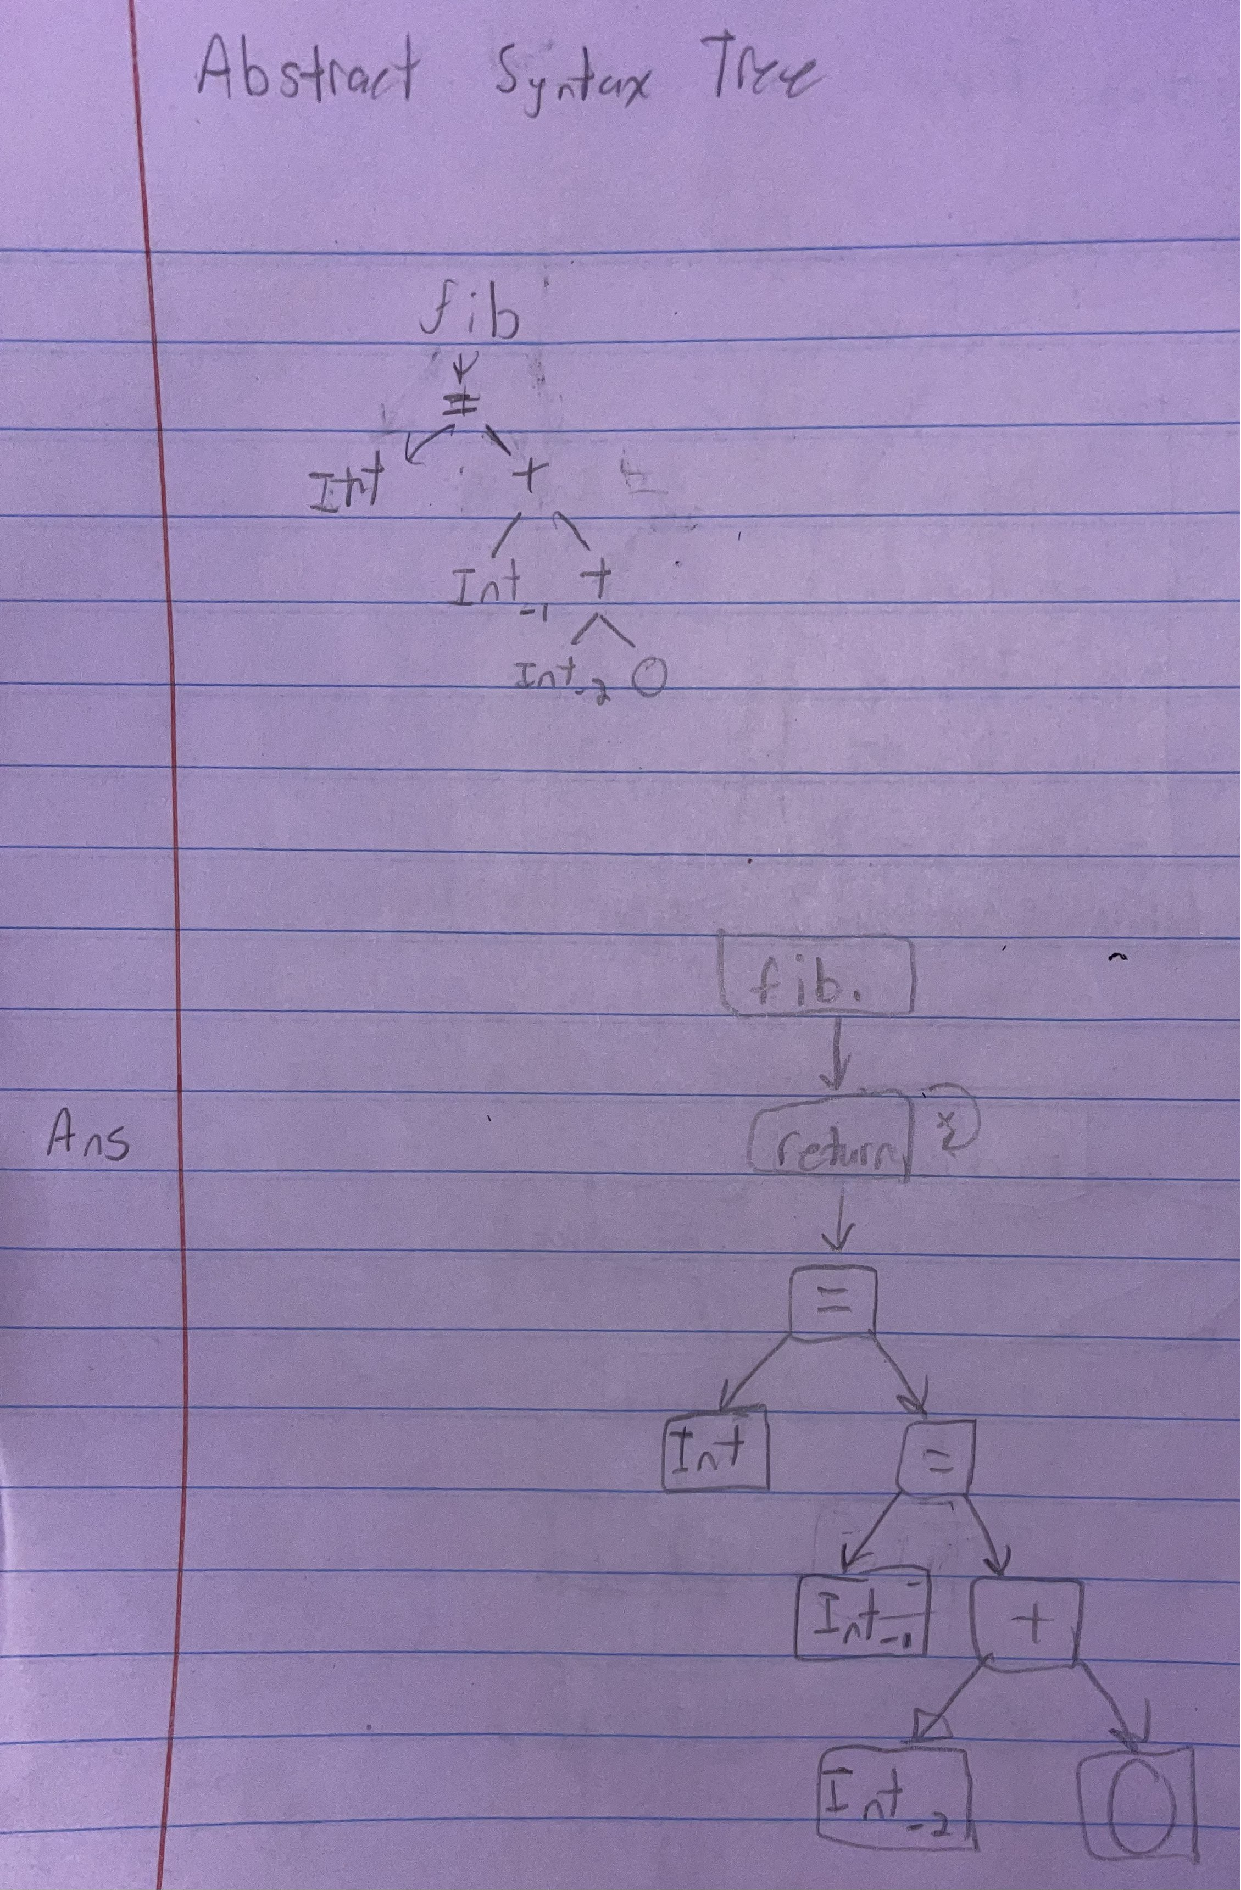
\includegraphics[width=15cm, height=20cm]{Week4P2.pdf}
\end{center}
\clearpage

\subsection{Week10}
Show, in the form of a proof tree, the steps taken by an interpreter evaluating the following program fragment.
\medskip\begin{center}
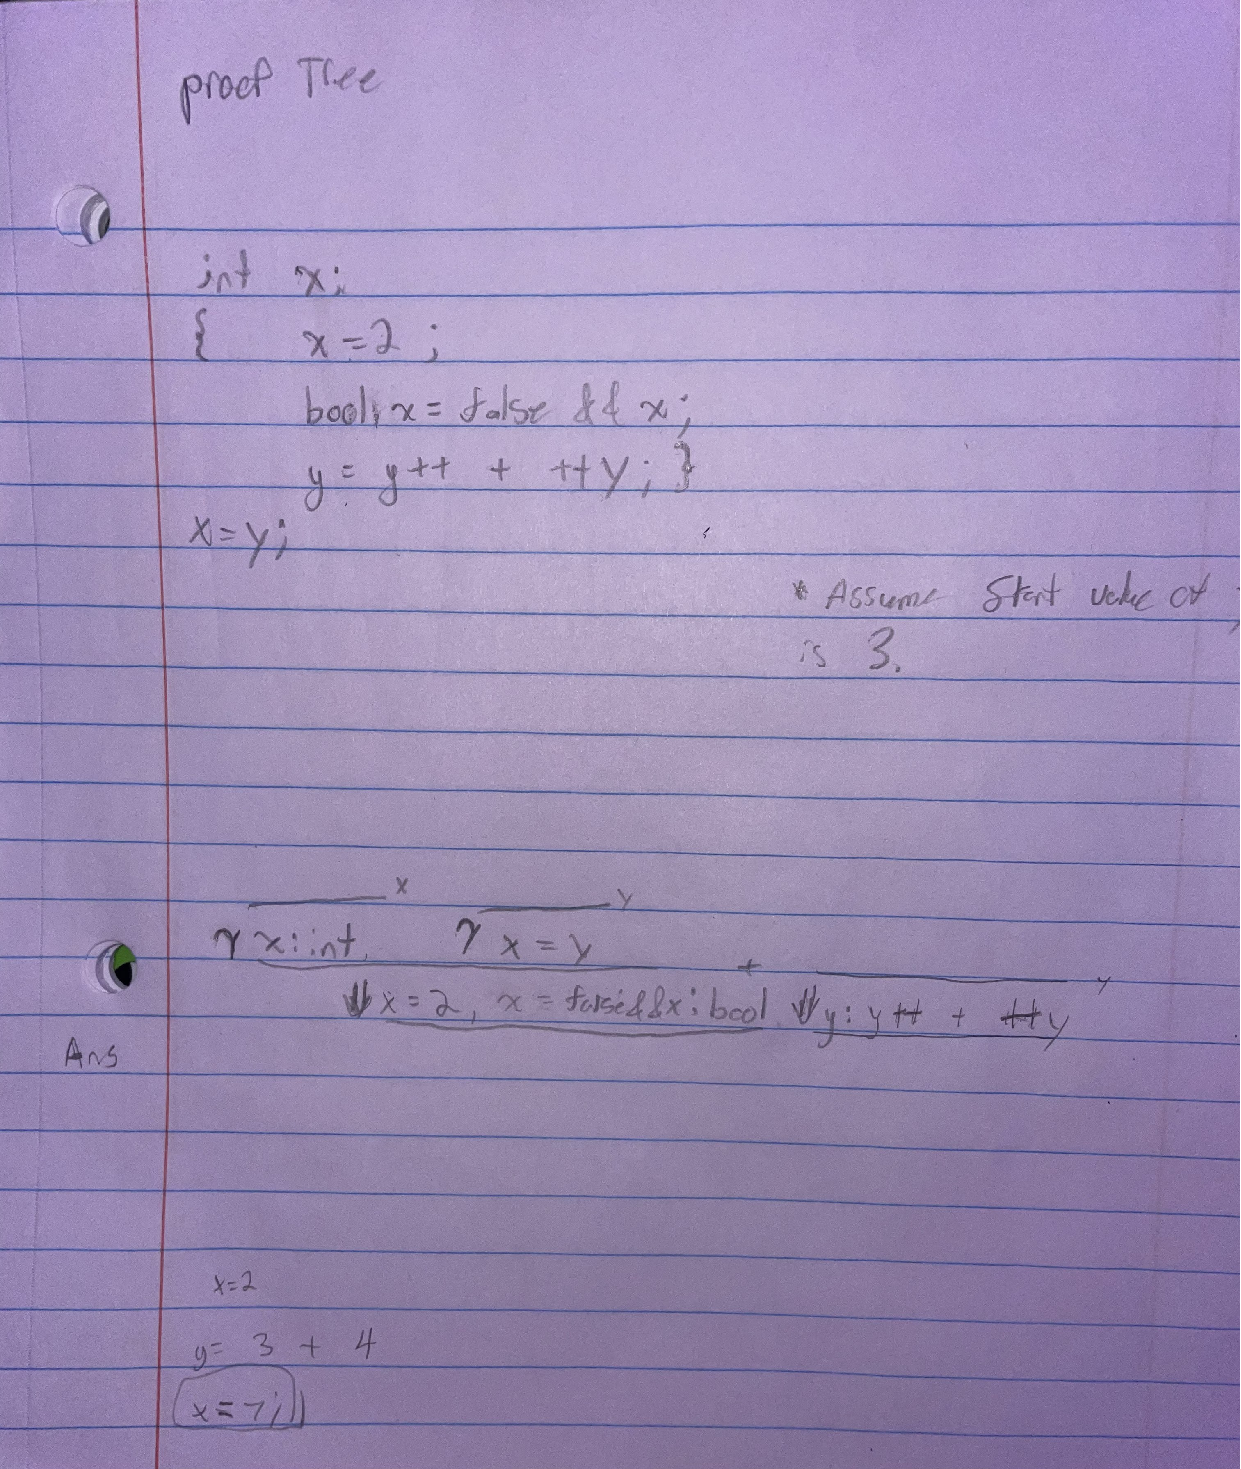
\includegraphics[width=15cm, height=20cm]{Week10.pdf}
\end{center}
\clearpage

\section{Project}

The project will be to compile code from a programming language of your choice to assembly and to explain the assembly code and compilation process using the knowledge your learned in this course. 


\medskip\noindent
Pro tips:
\begin{itemize}
\item Choose a compiled (not interpreted) programming language.
\item Choose a language that you find interesting anyway.
\item Start early.
\item Come to office hours. I have not run this part of the course before and I am really interested what you will find.
\end{itemize}
 
\section{Conclusions}\label{conclusions}

(approx 400 words)

In the conclusion, I want a critical reflection on the content of the course. Step back from the technical details. How does the course fit into the wider world of programming languages and software engineering?

\begin{thebibliography}{99}
\bibitem[HMU]{Hopcroft}
	John E. Hopcroft, Rajeev Motwani, Jeffrey D. Ullman:
\href{http://ce.sharif.edu/courses/94-95/1/ce414-2/resources/root/Text%20Books/Automata/John%20E.%20Hopcroft,%20Rajeev%20Motwani,%20Jeffrey%20D.%20Ullman-Introduction%20to%20Automata%20Theory,%20Languages,%20and%20Computations-Prentice%20Hall%20(2006).pdf}{Introduction to automata theory, languages, and computation,} 3rd Edition. Pearson international edition, Addison-Wesley 2007

\end{thebibliography}

\end{document}